
Usage:
\begin{longtable}[l]{m{15.795cm}}
\endhead
\endfoot
%\hline
\textbf{\ \ \ \ Solveur}\index{Solveur}\textbf{\_pression}\index{Solveur\_pression}
\ \textbf{Petsc}\index{Petsc}\textbf{ }\textit{\ Solver}\index{Solver} \{ \textbf{precond}
\textit{Precond}\index{Precond} \ 

\ \ \ \ \ \ \ \ \ \ \ \ \ \ \ \ \ \ \ \ \ \ \ \ \ \ \ \ \ \ \ \ \ \ \ \ \ \ \ \ \ \ \ \ \ \ \ \ \ \ \ \ \ \ \ \ \ \ \ \ \ [
\textbf{seuil} \textit{seuil} \ {\textbar} \textbf{nb\_it\_max} \textit{integer} ] \ 

\ \ \ \ \ \ \ \ \ \ \ \ \ \ \ \ \ \ \ \ \ \ \ \ \ \ \ \ \ \ \ \ \ \ \ \ \ \ \ \ \ \ \ \ \ \ \ \ \ \ \ \ \ \ \ \ \ \ \ \ \ [
\textbf{impr {\textbar} quiet} ] 

\ \ \ \ \ \ \ \ \ \ \ \ \ \ \ \ \ \ \ \ \ \ \ \ \ \ \ \ \ \ \ \ \ \ \ \ \ \ \ \ \ \ \ \ \ \ \ \ \ \ \ \ \ \ \ \ \ \ \ \ \ [
\textbf{save\_matrix {\textbar} read\_matrix}] 

\ \ \ \ \ \ \ \ \ \ \ \ \ \ \ \ \ \ \ \ \ \ \ \ \ \ \ \ \ \ \ \ \ \ \ \ \ \ \ \ \ \ \ \ \ \ \ \ \ \ \ \ \ \ \ \ \ \ \}
\\%\hline
\end{longtable}

\bigskip

\textit{Solver}\index{Solver}\textit{~}:\textit{ }Several solvers through PETSc API are available :

\ \ \textbf{GCP}\index{GCP} : Conjugate Gradient

\ \ \textbf{PIPECG : }Pipelined Conjugate Gradient (possible reduced CPU cost during massive parallel calculation due to
a single non-blocking reduction per iteration, if TRUST is built with a MPI-3 implementation). 

\ \ \textbf{GMRES} : Generalized Minimal Residual

\ \ \textbf{BICGSTAB} : Stabilized Bi-Conjugate Gradient\index{Gradient}

\textbf{\ \ IBICGSTAB}\index{IBICGSTAB}\textbf{ }: Improved version of previous one for massive parallel computations
(only a single global reduction operation instead of the usual 3 or 4).

\ \ \textbf{CHOLESKY} : Parallelized version of Cholesky\index{Cholesky} from MUMPS library. This solver accepts since
the 1.6.7 version an option to select a different ordering than the automatic selected one by MUMPS (and printed by
using the \textbf{impr} option). The possible choices are \textbf{Metis {\textbar} Scotch {\textbar} PT-Scotch
{\textbar} Parmetis}. The two last options can't only be used during a parallel calculation, whereas the two first are
available for sequential or parallel calculations. It seems that the CPU cost of A=LU factorization but also of the
backward/forward elimination steps may sometimes be reduced by selecting a different ordering than the default one.
Notice that this solver requires a huge amont of memory compared to iterative methods. To know how many RAM you will
need by core, then use the \textbf{impr} option to have detailled informations during the analysis phase and before the
factorisation phase (in the following output, you will learn that the largest memory is taken by the
0\textsuperscript{th} CPU with 108MB):

...

\ ** Rank of proc needing largest memory in IC facto \ \ \ \ \ \ \ : \ \ \ \ \ \ \ \ 0 

{\bfseries
\ ** Estimated corresponding MBYTES for IC facto \ \ \ \ \ \ \ \ \ \ \ : \ \ \ \ \ \ 108 }

...


\bigskip

Thanks to the following graph, you read that in order to solve for instance a flow on a mesh with 2.6e6 cells, you will
need to run a parallel calculation on 32 CPUs if you have cluster nodes with only 4GB/core (6.2GB*0.42\~{}2.6GB) :



\begin{center}
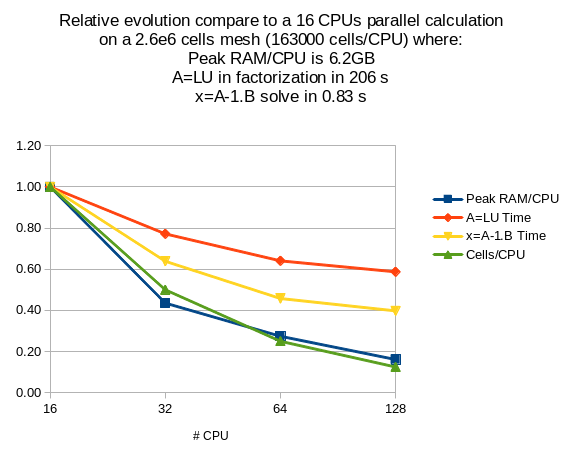
\includegraphics[width=15.212cm,height=12.266cm]{petsc_graph.png}
\end{center}
\textbf{\ \ CHOLESKY\_OUT\_OF\_CORE }: Same as the previous one but with a written LU decomposition of disc (save RAM
memory but add an extra CPU cost during Ax=B solve)

\textbf{\ \ CHOLESKY\_SUPERLU }: Parallelized Cholesky\index{Cholesky} from SUPERLU\_DIST library (less CPU and RAM
efficient than the previous one) 

\ \ \textbf{CHOLESKY\_PASTIX} : Parallelized Cholesky from PASTIX library

\ \ \textbf{CHOLESKY\_UMFPACK} : Sequential Cholesky from UMFPACK library (seems fast).

\textbf{\ \ \ \ \ \ \ \ \ \ CLI }\{ string \} : Command Line Interface\index{Interface}. Should be used only by advanced
users, \ to access the whole solver/preconditioners from the PETSC API. To find all the available options, run your
calculation with the -ksp\_view -help options:


\bigskip

trust datafile [N\index{N}] \ {}--ksp\_view --help

{\dots}

\textbf{Preconditioner (PC) Options}
-{}-{}-{}-{}-{}-{}-{}-{}-{}-{}-{}-{}-{}-{}-{}-{}-{}-{}-{}-{}-{}-{}-{}-{}-{}-{}-{}-{}-{}-{}-{}-{}-{}-{}-{}-{}-{}-{}-{}-{}-{}-{}-{}-{}-{}-{}-{}-{}-

\ \ {}-pc\_type\index{type} Preconditioner:(one of) none jacobi pbjacobi bjacobi sor lu shell mg

\ \ \ \ \ \ eisenstat ilu icc cholesky asm ksp composite redundant nn mat fieldsplit galerkin openmp spai hypre tfs
(PCSetType)

\ \ HYPRE preconditioner options

\ \ {}-pc\_hypre\_type\index{type} {\textless}pilut{\textgreater} (choose one of) pilut parasails boomeramg

\ \ HYPRE ParaSails Options

\ \ {}-pc\_hypre\_parasails\_nlevels {\textless}1{\textgreater}: Number of number of levels (None)

\ \ {}-pc\_hypre\_parasails\_thresh {\textless}0.1{\textgreater}: Threshold (None)

\ \ {}-pc\_hypre\_parasails\_filter {\textless}0.1{\textgreater}: filter (None)

\ \ {}-pc\_hypre\_parasails\_loadbal {\textless}0{\textgreater}: Load balance (None)

\ \ {}-pc\_hypre\_parasails\_logging: {\textless}FALSE{\textgreater} Print\index{Print} info to screen (None)

\ \ {}-pc\_hypre\_parasails\_reuse: {\textless}FALSE{\textgreater} Reuse nonzero pattern in preconditioner (None)

\ \ {}-pc\_hypre\_parasails\_sym {\textless}nonsymmetric{\textgreater} (choose one of) nonsymmetric SPD nonsymmetric,SPD

\textbf{Krylov Method (KSP) Options}
-{}-{}-{}-{}-{}-{}-{}-{}-{}-{}-{}-{}-{}-{}-{}-{}-{}-{}-{}-{}-{}-{}-{}-{}-{}-{}-{}-{}-{}-{}-{}-{}-{}-{}-{}-{}-{}-{}-{}-{}-{}-{}-{}-{}-{}-{}-{}-{}-

\ \ {}-ksp\_type\index{type} Krylov method:(one of) cg cgne stcg gltr richardson chebychev gmres tcqmr

\ \ \ \ \ \ bcgs bcgsl cgs tfqmr cr lsqr preonly qcg bicg fgmres minres symmlq lgmres lcd (KSPSetType)

\ \ {}-ksp\_max\_it {\textless}10000{\textgreater}: Maximum number of iterations (KSPSetTolerances)

\ \ {}-ksp\_rtol {\textless}0{\textgreater}: Relative decrease in residual norm (KSPSetTolerances)

\ \ {}-ksp\_atol {\textless}1e-12{\textgreater}: Absolute value of residual norm (KSPSetTolerances)

\ \ {}-ksp\_divtol {\textless}10000{\textgreater}: Residual norm increase cause divergence (KSPSetTolerances)

\ \ {}-ksp\_converged\_use\_initial\_residual\_norm: Use initial residual residual norm for computing relative
convergence

\ \ {}-ksp\_monitor\_singular\_value {\textless}stdout{\textgreater}: Monitor singular values (KSPMonitorSet)

\ \ {}-ksp\_monitor\_short {\textless}stdout{\textgreater}: Monitor preconditioned residual norm with fewer digits
(KSPMonitorSet)

\ \ {}-ksp\_monitor\_draw: Monitor graphically preconditioned residual norm (KSPMonitorSet)

\ \ {}-ksp\_monitor\_draw\_true\_residual: Monitor graphically true residual norm (KSPMonitorSet)


\bigskip

Example to use the multigrid method as a solver, not only as a preconditioner:

\textbf{Solveur}\index{Solveur}\textbf{\_pression}\index{Solveur\_pression} \textbf{Petsc}\index{Petsc} \textbf{CLI} \{
-ksp\_type\index{type} richardson -pc\_type hypre -pc\_hypre\_type boomeramg -ksp\_atol 1.e-7 \}


\bigskip


\bigskip

\textit{Precond}\index{Precond}\textit{~}: Several preconditioners are available :

\textit{\ \ }\textbf{NULL}\index{NULL} \{ \} : No preconditioner used

\ \ \textbf{BLOCK\_JACOBI\_ICC }\{\textbf{ level }k \textbf{ordering} \textbf{natural} {\textbar} \textbf{rcm} \} :
Incomplete Cholesky\index{Cholesky} factorization for symmetric matrix with the PETSc implementation. The integer k is
the factorization level (default value, 1). In parallel, the factorization is done by block (one per processor by
default). The ordering of the local\index{local} matrix is \textbf{natural} by default, but \textbf{rcm} ordering,
which reduces the bandwith of the local matrix, may interestingly improves the quality of the decomposition and reduces
the number of iterations.

\ \ \textbf{SSOR}\index{SSOR} \{ \textbf{omega} double \} : Symmetric Successive Over Relaxation algorithm.
\textbf{omega} (default value, 1.5) defines the relaxation factor. 

\textbf{\ \ EISENTAT }\{ \textbf{omega }double \} : SSOR\index{SSOR} version with Eisenstat trick which reduces the
number of computations and thus CPU cost

\textbf{\ \ SPAI }\{\textbf{ level }nlevels \textbf{epsilon} thresh \} : Spai\index{Spai} Approximate Inverse algorithm
from Parasails Hypre library. Two parameters are available, nlevels and thresh.

\ \ \textbf{PILUT} \{ \textbf{level} k \textbf{epsilon} thresh \}: Dual Threashold Incomplete LU factorization. The
integer k is the factorization level and \textbf{epsilon} is the drop tolerance.

\ \ \textbf{DIAG} \{ \ \} : Diagonal (Jacobi) preconditioner.

\ \ \textbf{BOOMERAMG} \{ \} : Multigrid preconditioner (no option is available yet, look at CLI command and
Petsc\index{Petsc} documentation to try other options).


\bigskip

\textbf{seuil}\textit{ }corresponds to the iterative solver convergence value. The iterative solver converges when the
Euclidean residue standard {\textbar}{\textbar}Ax-B{\textbar}{\textbar} is less than the value \textit{seuil}. 


\bigskip

\textbf{nb\_it\_max} integer : In order to specify a given number of iterations instead of a condition on the residue
with the keyword \textbf{seuil}. May be useful when defining a PETSc solver for the implicit time scheme where
convergence is very fast: 5 or less iterations seems enough.


\bigskip

\textbf{impr} is the keyword which is used to request display of the Euclidean residue standard each time this iterates
through the conjugated gradient (display to the standard outlet).


\bigskip

\textbf{quiet} is a keyword which is used to not displaying any outputs of the solver.


\bigskip

\textbf{save\_matrix{\textbar}read\_matrix} are the keywords to save{\textbar}read into a file the constant matrix A of
the linear system Ax=B solved (eg: matrix from the pressure linear system for an incompressible flow). It is useful
when you want to minimize the MPI communications on massive parallel calculation. Indeed, in VEF discretization, the
overlapping width (generaly 2, specified with the \textbf{largeur\_joint} option in the partition keyword
\textbf{partition}) can be reduced to 1, once the matrix has been properly assembled and saved. The cost of the MPI
communications in TRUST itself (not in PETSc) will be reduced with length messages divided by 2. So the strategy is:

I) Partition your VEF mesh with a \textbf{largeur\_joint }value of 2

II) Run your parallel calculation on 0 time step, to build and save the matrix with the \textbf{save\_matrix} option. A
file named \textit{Matrix\_NBROWS\_rows\_NCPUS\_cpus.petsc} will be saved to the disc (where NBROWS is the number of
rows of the matrix and NCPUS the number of CPUs used). 

III) Partition your VEF mesh with a \textbf{largeur\_joint} value of 1

IV) Run your parallel calculation completly now and substitute the \textbf{save\_matrix} option by the
\textbf{read\_matrix} option. Some interesting gains have been noticed when the cost of linear system solve with PETSc
is small compared to all the other operations. 


\bigskip


\bigskip

{\bfseries\itshape
TIPS:}

A) Solver\index{Solver} for symmetric linear systems (e.g: Pressure system from Navier Stokes equation):

{}-The \textbf{CHOLESKY} parallel solver is from MUMPS library. It offers better performance than all others solvers if
you have enough RAM for your calculation. A parallel calculation on a cluster with 4GBytes on each processor, 40000
cells/processor seems the upper limit. Seems to be very slow to initialize above 500 cpus/cores.


\bigskip

{}-When running a parallel calculation with a high number of cpus/cores (typically more than 500) where preconditioner
scalabilty is the key for CPU performance, consider \textbf{BICGSTAB }with \textbf{BLOCK\_JACOBI\_ICC(1)} as
preconditioner or if not converges, \textbf{GCP}\index{GCP}\textbf{ }with\textbf{ BLOCK\_JACOBI\_ICC(1) }as
preconditioner.


\bigskip

{}-For other situations, the first choice should be \textbf{GCP}\index{GCP}\textbf{/SSOR}\index{SSOR}. In order to fine
tune the solver choice, each one of the previous list should be considered. Indeed, the CPU speed of a solver depends
of a lot of parameters. You may give a try to the \textbf{OPTIMAL} solver to help you to find the fastest solver on
your study. 


\bigskip

B) Solver\index{Solver} for non symmetric linear systems (e.g.: Implicit schemes):

The \textbf{BICGSTAB/DIAG }solver seems to offer the best performances.


\bigskip

Additional information is available into the PETSC documentation available there:
\textbf{\$TRUST\_ROOT/lib/src/LIBPETSC/petsc/*/docs/manual.pdf}
